\section{Durchführung}
\label{sec:Durchführung}
Damit Dichte, Rauigkeit und Dicke eines Polysterolfilms auf einem Siliziumwafer bestimmt werden können, muss in einem ersten Schritt die Messapparatur
justiert und kalibriert werden.
Der verwendete Versuchsaufbau ist in \autoref{fig:Aufbau} gezeigt, die Datennahme erfolgt über einen angeschlossenen Computer.

\begin{figure}
    \centering
    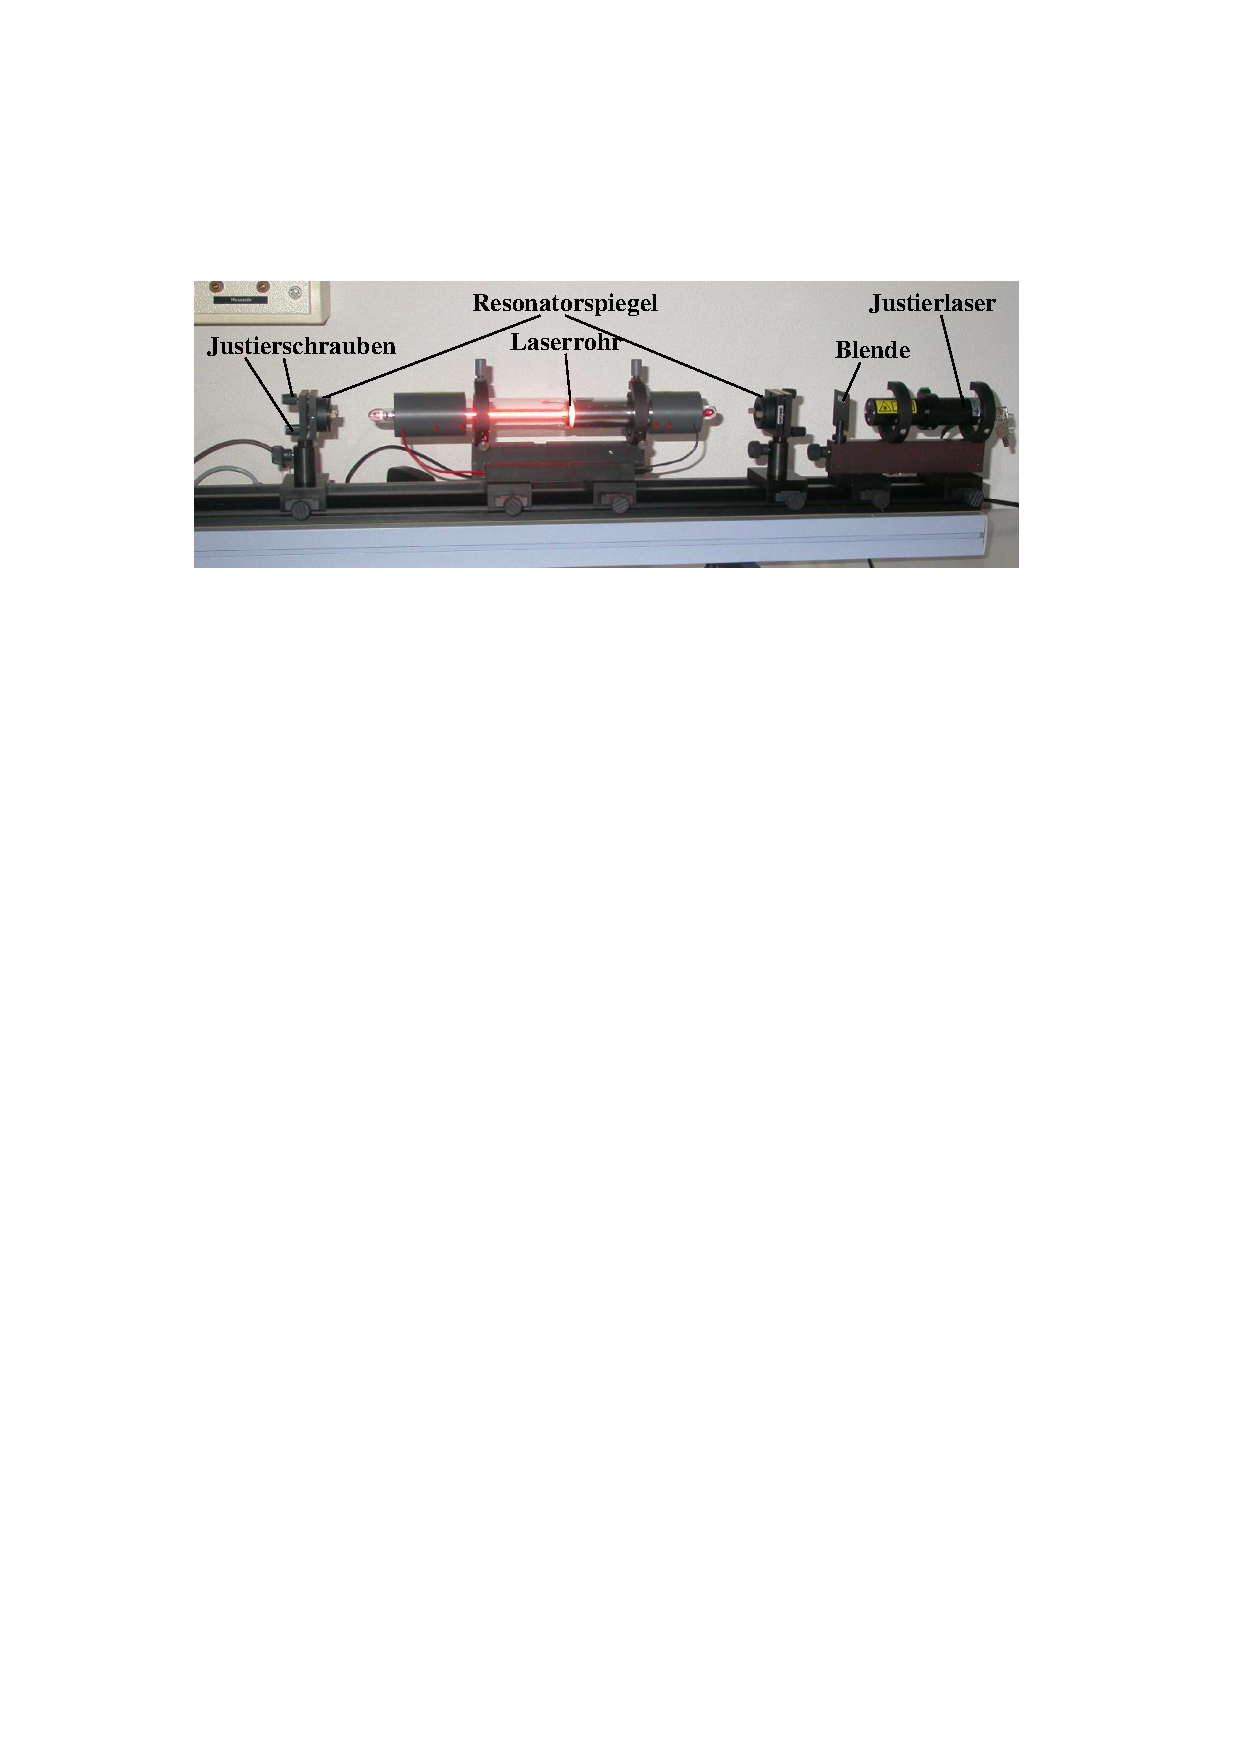
\includegraphics[width=0.9\textwidth]{content/pics/Aufbau.pdf}
    \caption{Bild des verwendeten Diffraktometers. Zu sehen sind \textbf{(a)} Röntgenröhre, \textbf{(b)} Probe, \textbf{(c)} Detektor, \textbf{(d)} xyz-Messtisch.}
    \label{fig:Aufbau}
\end{figure}

\subsection{Justierung der Messapparatur}

\subsection{Vermessung der Probe}